%% Copernicus Publications Manuscript Preparation Template for LaTeX Submissions
%% ---------------------------------
%% This template should be used for copernicus.cls
%% The class file and some style files are bundled in the Copernicus Latex Package, which can be downloaded from the different journal webpages.
%% For further assistance please contact Copernicus Publications at: production@copernicus.org
%% https://publications.copernicus.org/for_authors/manuscript_preparation.html

%% copernicus_rticles_template (flag for rticles template detection - do not remove!)

%% Please use the following documentclass and journal abbreviations for discussion papers and final revised papers.

%% 2-column papers and discussion papers
\documentclass[, manuscript]{copernicus}



%% Journal abbreviations (please use the same for discussion papers and final revised papers)


% Advances in Geosciences (adgeo)
% Advances in Radio Science (ars)
% Advances in Science and Research (asr)
% Advances in Statistical Climatology, Meteorology and Oceanography (ascmo)
% Annales Geophysicae (angeo)
% Archives Animal Breeding (aab)
% ASTRA Proceedings (ap)
% Atmospheric Chemistry and Physics (acp)
% Atmospheric Measurement Techniques (amt)
% Biogeosciences (bg)
% Climate of the Past (cp)
% DEUQUA Special Publications (deuquasp)
% Drinking Water Engineering and Science (dwes)
% Earth Surface Dynamics (esurf)
% Earth System Dynamics (esd)
% Earth System Science Data (essd)
% E&G Quaternary Science Journal (egqsj)
% European Journal of Mineralogy (ejm)
% Fossil Record (fr)
% Geochronology (gchron)
% Geographica Helvetica (gh)
% Geoscience Communication (gc)
% Geoscientific Instrumentation, Methods and Data Systems (gi)
% Geoscientific Model Development (gmd)
% History of Geo- and Space Sciences (hgss)
% Hydrology and Earth System Sciences (hess)
% Journal of Bone and Joint Infection (jbji)
% Journal of Micropalaeontology (jm)
% Journal of Sensors and Sensor Systems (jsss)
% Magnetic Resonance (mr)
% Mechanical Sciences (ms)
% Natural Hazards and Earth System Sciences (nhess)
% Nonlinear Processes in Geophysics (npg)
% Ocean Science (os)
% Polarforschung - Journal of the German Society for Polar Research (polf)
% Primate Biology (pb)
% Proceedings of the International Association of Hydrological Sciences (piahs)
% Scientific Drilling (sd)
% SOIL (soil)
% Solid Earth (se)
% The Cryosphere (tc)
% Weather and Climate Dynamics (wcd)
% Web Ecology (we)
% Wind Energy Science (wes)

%% Please DO NOT add additional packages or LaTeX commands to the template. They
%% are not supported by Coperncius. LaTeX packages already
%% included in the copernicus.cls are:
%\usepackage[german, english]{babel}
%\usepackage{tabularx}
%\usepackage{cancel}
%\usepackage{multirow}
%\usepackage{supertabular}
%\usepackage{algorithmic}
%\usepackage{algorithm}
%\usepackage{amsthm}
%\usepackage{float}
%\usepackage{subfig}
%\usepackage{rotating}

% Pandoc citation processing

% The "Technical instructions for LaTex" by Copernicus require _not_ to insert any additional packages.
%

\begin{document}

\title{Template for preparing your manuscript submission to Copernicus
journals using RMarkdown}


\Author[1, *]{Daniel}{Nüst}
\Author[2]{Josiah}{Carberry}
\Author[1, *]{Markus}{Konkol}
\Author[3, †]{Nikolaus}{Copernicus}


\affil[1]{Institute for Geoinformatics, University of Münster, 48149
Münster, Germany}
\affil[2]{Psychoceramics, Wesleyan University, Middletown, CT, United
States}
\affil[3]{University of Ferrara, Ferrara, Italy}
\affil[†]{deceased, 24 May 1543}
\affil[*]{These authors contributed equally to this work.}

\runningtitle{R Markdown Template for Copernicus}

\runningauthor{Nüst et al.}


\correspondence{Daniel\ Nüst\ (daniel.nuest@uni-muenster.de)}



\received{}
\pubdiscuss{} %% only important for two-stage journals
\revised{}
\accepted{}
\published{}

%% These dates will be inserted by Copernicus Publications during the typesetting process.


\firstpage{1}

\maketitle


\begin{abstract}
The abstract goes here. It can also be on \emph{multiple lines}.
\end{abstract}


\copyrightstatement{The author's copyright for this publication is
transferred to institution/company.}


\introduction[Introduction]

Introduction text goes here. You can change the name of the section if
necessary using
\texttt{\textbackslash{}introduction{[}modified\ heading{]}}.

The following settings can or must be configured in the header of this
file and are bespoke for Copernicus manuscripts:

\begin{itemize}
\item
  The \texttt{journal} you are submitting to using the official
  abbreviation. You can use the function
  \texttt{rticles::copernicus\_journal\_abbreviations(name\ =\ \textquotesingle{}...\textquotesingle{})}
  to search the existing journals.
\item
  Specific sections of the manuscript:

  \begin{itemize}
  \item
    \texttt{running} with \texttt{title} and \texttt{author}
  \item
    \texttt{competinginterests}
  \item
    \texttt{copyrightstatement} (optional)
  \item
    \texttt{availability} (strongly recommended if any used), one of
    \texttt{code}, \texttt{data}, or \texttt{codedata}
  \item
    \texttt{authorcontribution}
  \item
    \texttt{disclaimer}
  \item
    \texttt{acknowledgements}
  \end{itemize}
\end{itemize}

See the defaults and examples from the skeleton and the official
Copernicus documentation for details.

\textbf{Please note:} Per
\href{https://publications.copernicus.org/for_authors/manuscript_preparation.html}{their
guidelines}, Copernicus does not support additional \LaTeX{} packages or
new \LaTeX{} commands than those defined in their \texttt{.cls} file.
This means that you cannot add any extra dependencies and a warning will
be thrown if so.\\
This extends to syntax highlighting of source code. Therefore this
template sets the parameter \texttt{highlight} in the YAML header to
\texttt{NULL} to deactivate Pandoc syntax highlighter. This prevent
addition of external packages for highlighting inserted by Pandoc.
However, it might be desirable to have syntax highlight available in
preprints or for others reasons. Please see
\texttt{?rmarkdown::pdf\_document} for available options to activate
highlighting.

\textbf{Important}: Always double-check with the official manuscript
preparation guidelines at
\url{https://publications.copernicus.org/for_authors/manuscript_preparation.html},
especially the sections ``Technical instructions for LaTeX'' and
``Manuscript composition''. Please contact Daniel Nüst,
\texttt{daniel.nuest@uni-muenster.de}, with any problems.

\section{Content section one}

\subsection{Subsection Heading Here}

Subsection text here.

\subsubsection{Subsubsection Heading Here}

Subsubsection text here.

\section{Content section with citations}

See the
\href{http://rmarkdown.rstudio.com/authoring_bibliographies_and_citations.html}{R
Markdown docs for bibliographies and citations}.

Copernicus supports biblatex and a sample bibliography is in file
\texttt{sample.bib}. Read and
\citep[see][]{kingRoleClimateVariability2020b}.

\section{Content section with R code chunks}

You should always use \texttt{echo\ =\ FALSE} on R Markdown code blocks
as they add formatting and styling not desired by Copernicus. The hidden
workflow results in 42.

You can add verbatim code snippets without extra styles by using
\texttt{\textasciigrave{}\textasciigrave{}\textasciigrave{}} without
additional instructions. \cite{ahlstromLargeInfluenceClimate2017}

\begin{verbatim}
sum <- 1 + 41
\end{verbatim}

\section{Content section with list}

If you want to insert a list, you must

\begin{itemize}
\item
  leave
\item
  empty lines
\item
  between each list item
\end{itemize}

because the \texttt{\textbackslash{}tightlist} format used by R Markdown
is not supported in the Copernicus template. Example:

\begin{verbatim}
- leave

- empty lines

- between each list item
\end{verbatim}

\section{Examples from the official template}

\subsection{FIGURES}

When figures and tables are placed at the end of the MS (article in
one-column style), please add \clearpage between bibliography and first
table and/or figure as well as between each table and/or figure.

\subsubsection{ONE-COLUMN FIGURES}

Include a 12cm width figure of Nikolaus Copernicus from
\href{https://en.wikipedia.org/wiki/File:Nikolaus_Kopernikus.jpg}{Wikipedia}
with caption using R Markdown.

\begin{figure}
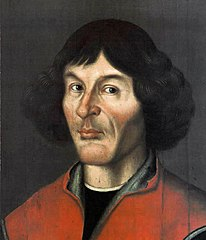
\includegraphics[width=8.3cm]{Nikolaus_Kopernikus} \caption{one column figure}\label{fig:unnamed-chunk-2}
\end{figure}

\subsubsection{TWO-COLUMN FIGURES}

You can also include a larger figure.

\begin{figure}
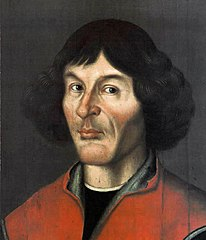
\includegraphics[width=12cm]{Nikolaus_Kopernikus} \caption{two column figure}\label{fig:unnamed-chunk-3}
\end{figure}

\subsection{TABLES}

You can ad \LaTeX table in an R Markdown document to meet the template
requirements.

\subsubsection{ONE-COLUMN TABLE}

\begin{table}[t]
\caption{TEXT}
\begin{tabular}{l c r}
\tophline

a & b & c \\
\middlehline
1 & 2 & 3 \\

\bottomhline
\end{tabular}
\belowtable{Table Footnotes}
\end{table}

\subsubsection{TWO-COLUMN TABLE}

\begin{table*}[t]
\caption{TEXT}
\begin{tabular}{l c r}
\tophline

a & b & c \\
\middlehline
1 & 2 & 3 \\

\bottomhline
\end{tabular}
\belowtable{Table footnotes}
\end{table*}

\subsection{MATHEMATICAL EXPRESSIONS}

All papers typeset by Copernicus Publications follow the math
typesetting regulations given by the IUPAC Green Book (IUPAC:
Quantities, Units and Symbols in Physical Chemistry, 2nd Edn., Blackwell
Science, available at:
http://old.iupac.org/publications/books/gbook/green\_book\_2ed.pdf,
1993).

Physical quantities/variables are typeset in italic font (t for time, T
for Temperature)

Indices which are not defined are typeset in italic font (x, y, z, a, b,
c)

Items/objects which are defined are typeset in roman font (Car A, Car B)

Descriptions/specifications which are defined by itself are typeset in
roman font (abs, rel, ref, tot, net, ice)

Abbreviations from 2 letters are typeset in roman font (RH, LAI)

Vectors are identified in bold italic font using \vec{x}

Matrices are identified in bold roman font

Multiplication signs are typeset using the LaTeX commands
\texttt{\textbackslash{}times} (for vector products, grids, and
exponential notations) or \texttt{\textbackslash{}cdot}

The character * should not be applied as mutliplication sign

\subsection{EQUATIONS}

\subsubsection{Single-row equation}

Unnumbered equations (i.e.~using \texttt{\$\$} and getting inline
preview in RStudio) are not supported by Copernicus.

\begin{equation}
1 \times 1 \cdot 1 = 42
\end{equation}

\begin{equation}
A = \pi r^2
\end{equation}

\begin{equation}
x=\frac{2b\pm\sqrt{b^{2}-4ac}}{2c}.  
\end{equation}

\subsubsection{Multiline equation}

\begin{align}
& 3 + 5 = 8\\
& 3 + 5 = 8\\
& 3 + 5 = 8
\end{align}

\subsection{MATRICES}

\[
\begin{matrix}
x & y & z\\
x & y & z\\
x & y & z\\
\end{matrix}
\]

\subsection{ALGORITHM/PROGRAMMING CODE}

If you want to use algorithms, you need to make sure yourself that the
\LaTeX packages \texttt{algorithms} and \texttt{algorithmicx} are
installed so that \texttt{algorithm.sty} respectively
\texttt{algorithmic.sty} can be loaded by the Copernicus template. Both
need to be available through your preferred \LaTeX{} distribution. With
TinyTeX (or TeX Live), you can do so by running
\texttt{tinytex::tlmgr\_install(c("algorithms",\ "algorithmicx"))}

\begin{verbatim}
## tlmgr update --all --self
\end{verbatim}

\begin{verbatim}
## tlmgr install algorithms algorithmicx
\end{verbatim}

Copernicus staff will no accept any additional packages from your LaTeX
source code, so please stick to these two acceptable packages. They are
needed to use the example below

\begin{algorithm}
\caption{Algorithm Caption}
\label{a1}
\begin{algorithmic}
\STATE $i\gets 10$
\IF {$i\geq 5$} 
        \STATE $i\gets i-1$
\ELSE
        \IF {$i\leq 3$}
                \STATE $i\gets i+2$
        \ENDIF
\ENDIF
\end{algorithmic}
\end{algorithm}

\subsection{CHEMICAL FORMULAS AND REACTIONS}

For formulas embedded in the text, please use
\texttt{\textbackslash{}chem\{\}}, e.g.~\chem{A \rightarrow B}.

The reaction environment creates labels including the letter R,
i.e.~(R1), (R2), etc.

\begin{itemize}
\item
  \texttt{\textbackslash{}rightarrow} should be used for normal
  (one-way) chemical reactions
\item
  \texttt{\textbackslash{}rightleftharpoons} should be used for
  equilibria
\item
  \texttt{\textbackslash{}leftrightarrow} should be used for resonance
  structures
\end{itemize}

\begin{reaction}
A \rightarrow B \\
\end{reaction}
\begin{reaction}
Coper \rightleftharpoons nicus \\
\end{reaction}
\begin{reaction}
Publi \leftrightarrow cations
\end{reaction}

\subsection{PHYSICAL UNITS}

Please use \texttt{\textbackslash{}unit\{\}} (allows to save the
math/\texttt{\$} environment) and apply the exponential notation, for
example \(3.14\,\unit{km\,h^{-1}}\) (using LaTeX mode:
\texttt{\textbackslash{}(\ 3.14\textbackslash{},\textbackslash{}unit\{...\}\ \textbackslash{})})
or \unit{0.872\,m\,s^{-1}} (using only
\texttt{\textbackslash{}unit\{0.872\textbackslash{},m\textbackslash{},s\^{}\{-1\}\}}).

\conclusions[Conclusions]

The conclusion goes here. You can modify the section name with
\texttt{\textbackslash{}conclusions{[}modified\ heading\ if\ necessary{]}}.



\codedataavailability{use this to add a statement when having data sets
and software code
available} %% use this section when having data sets and software code available

\sampleavailability{use this section when having geoscientific samples
available} %% use this section when having geoscientific samples available

\videosupplement{use this section when having video supplements
available} %% use this section when having geoscientific samples available

%%%%%%%%%%%%%%%%%%%%%%%%%%%%%%%%%%%%%%%%%%
%% optional

%%%%%%%%%%%%%%%%%%%%%%%%%%%%%%%%%%%%%%%%%%
\appendix
\section{Figures and tables in appendices}

Regarding figures and tables in appendices, the following two options
are possible depending on your general handling of figures and tables in
the manuscript environment:

\subsection{Option 1}

If you sorted all figures and tables into the sections of the text,
please also sort the appendix figures and appendix tables into the
respective appendix sections. They will be correctly named
automatically.

\subsection{Option 2}

If you put all figures after the reference list, please insert appendix
tables and figures after the normal tables and figures.

To rename them correctly to A1, A2, etc., please add the following
commands in front of them: \texttt{\textbackslash{}appendixfigures}
needs to be added in front of appendix figures
\texttt{\textbackslash{}appendixtables} needs to be added in front of
appendix tables

Please add \texttt{\textbackslash{}clearpage} between each table and/or
figure. Further guidelines on figures and tables can be found below.
\noappendix

%%%%%%%%%%%%%%%%%%%%%%%%%%%%%%%%%%%%%%%%%%
\authorcontribution{Daniel wrote the package. Josiah thought about
poterry. Markus filled in for a second author.} %% optional section

%%%%%%%%%%%%%%%%%%%%%%%%%%%%%%%%%%%%%%%%%%
\competinginterests{The authors declare no competing
interests.} %% this section is mandatory even if you declare that no competing interests are present

%%%%%%%%%%%%%%%%%%%%%%%%%%%%%%%%%%%%%%%%%%
\disclaimer{We like Copernicus.} %% optional section

%%%%%%%%%%%%%%%%%%%%%%%%%%%%%%%%%%%%%%%%%%
\begin{acknowledgements}
Thanks to the rticles contributors!
\end{acknowledgements}

%% REFERENCES
%% DN: pre-configured to BibTeX for rticles

%% The reference list is compiled as follows:
%%
%% \begin{thebibliography}{}
%%
%% \bibitem[AUTHOR(YEAR)]{LABEL1}
%% REFERENCE 1
%%
%% \bibitem[AUTHOR(YEAR)]{LABEL2}
%% REFERENCE 2
%%
%% \end{thebibliography}

%% Since the Copernicus LaTeX package includes the BibTeX style file copernicus.bst,
%% authors experienced with BibTeX only have to include the following two lines:
%%
\bibliographystyle{copernicus}
\bibliography{test.bib}
%%
%% URLs and DOIs can be entered in your BibTeX file as:
%%
%% URL = {http://www.xyz.org/~jones/idx_g.htm}
%% DOI = {10.5194/xyz}


%% LITERATURE CITATIONS
%%
%% command                        & example result
%% \citet{jones90}|               & Jones et al. (1990)
%% \citep{jones90}|               & (Jones et al., 1990)
%% \citep{jones90,jones93}|       & (Jones et al., 1990, 1993)
%% \citep[p.~32]{jones90}|        & (Jones et al., 1990, p.~32)
%% \citep[e.g.,][]{jones90}|      & (e.g., Jones et al., 1990)
%% \citep[e.g.,][p.~32]{jones90}| & (e.g., Jones et al., 1990, p.~32)
%% \citeauthor{jones90}|          & Jones et al.
%% \citeyear{jones90}|            & 1990

\end{document}
